\documentclass[14pt]{beamer}

%% Fonts and encodings
\usepackage{multicol}
\usepackage{mathabx}
\usepackage[scaled]{helvet}
\usepackage{color}
\usepackage{lmodern}
\usepackage{eulervm}
\usepackage{wasysym}
\usefonttheme[onlymath]{serif}
\usefonttheme{professionalfonts}
\usefonttheme{structurebold}
\hypersetup{backref}
\usepackage{bm}
%\usepackage[utf8x]{inputenc}

\usepackage{ctex}
\usepackage{xeCJK}
\setCJKmainfont[ItalicFont={Adobe Kaiti Std},
                BoldFont={Adobe Heiti Std}]{Adobe Song Std}
\setCJKsansfont{Adobe Heiti Std}
\setCJKmonofont{Adobe Fangsong Std}



%% Color & Theme
\definecolor{SUblue}{RGB}{0,0,180}
\usecolortheme[RGB={0,0,180}]{structure}
\usetheme{Boadilla}
\setbeamertemplate{navigation symbols}{}
\setbeamerfont{title}{size=\large}
\setbeamerfont{frametitle}{size=\normalsize}
\setbeamerfont{framesubtitle}{size=\small, shape =$\color{violet}{\looparrowdownright}~$}
\setbeamercolor{title}{fg=white, bg= SUblue!75!green}
\setbeamercolor{framesubtitle}{fg=violet}

%% Reduce the left margin
\setlength{\leftmargini}{5pt}
\setbeamertemplate{frametitle}
{
\raggedright\insertframetitle%
}


\title[Covariate-dependent copulas]{{\textbf{Introduction to
      covariate-dependent\\ copula modeling
\footnote{\tiny{Based on paper \textbf{Li, F. (2012), Modeling covariate-contingent correlation and tail-dependence with copulas}.}}
}}}

\author[Feng Li]{\textbf{Feng Li}}
\institute[Stockholm University]{\textbf{Department of
    Statistics, Stockholm University}}
\date{\color{SUblue}{ \textbf{March, 2013}}}



\begin{document}

%% Title page

%% Outline
% \section*{Outline of the talk}
% \begin{frame}
%   \frametitle{Outline of the talk}
%   \addtocounter{framenumber}{-1}
%   \tableofcontents
% \end{frame}

\section*{简要个人介绍}
\begin{frame}[plain]
  \frametitle{李丰:\color{violet}{瑞典斯德哥尔摩大学统计系}}
  \addtocounter{framenumber}{-2}

  \begin{itemize}
  \item [] \textbf{研究兴趣}:

    贝叶斯理论,计量经济学,预测方法,多元模型

  \item [] \textbf{博士论文}:

    \emph{Flexible Bayesian Regression Density Estimation}\\
    (\emph{柔性贝叶斯回归密度估计})

  \item [] \textbf{教过课程}:

    回归分析,时间序列,统计计算,贝叶斯方法
  \end{itemize}

\end{frame}

\begin{frame}[plain]
  \addtocounter{framenumber}{0}
  \titlepage
\end{frame}


%%%%%%%%%%%%%%%%%%%%%%%%%%%%%%%%%%%%%%%%%%%%%%%%%%%%%%%%%%%%%%%%%%%%%%%%%%%%%%%%
%% The main slides
%%%%%%%%%%%%%%%%%%%%%%%%%%%%%%%%%%%%%%%%%%%%%%%%%%%%%%%%%%%%%%%%%%%%%%%%%%%%%%%%

\section{Introduction to copulas}
\begin{frame}
  % \frametitle{Introduction to copulas}
  \frametitle{What is a copula?}
  \begin{itemize}
  \item The word ``\textbf{copula}'' means \textbf{linking}.
  \item \textbf{Sklar's theorem (1959)}

    Let $H$ be a multi-dimensional distribution function with marginal
    distribution functions $F_1(x_1),...,F_M(x_M)$. Then there exists a
    function $C$ (\textbf{copula function}) such that
    \begin{equation*}
      \begin{split}
        &H(x_1,...,x_M)=  C(F_1(x_1),...,F_M(x_M))\\
        &=C\left(\int_{-\infty}^{x_1}f(z_1)dz_1,...,\int_{-\infty}^{x_M}f(z_M)dz_M\right)=C(\bm{u}_1,...,\bm{u}_M).
      \end{split}
    \end{equation*}

  \end{itemize}
\end{frame}

\begin{frame}
  %\frametitle{Introduction to copulas}
  \frametitle{Some arbitrary examples}
  \begin{itemize}

  \item If $X_1,...,X_M$ are independent, and iff $C$ is a product copula, then
    \begin{equation*}
      C(F_1(x_1),...,F_M(x_M))=\prod \nolimits _{i=1}^{M} F_i(x_i)
    \end{equation*}

  \item The bivariate Gaussian copula
    \begin{equation*}
      \begin{split}
        &C(u_1,u_2,\rho)=\bm{\Phi}_2(\Phi^{-1}(u_1),\Phi^{-1}(u_2),\rho)\\
        % &= \int_{-\infty}^{\Phi^{-1}(u_1)}\int_{-\infty}^{\Phi^{-1}(u_2)}
        % \frac{1}{2\pi\sqrt{1-\rho^2}}\exp\left\{- \frac{z_1^2-2\rho z_1z_2+z_2^2}{2(1-\rho^2)} \right\}\mathrm{d}z_1\mathrm{d}z_2
      \end{split}
    \end{equation*}

  \item The multivariate probit model is a simple Gaussian copula model,
    with univariate probit regressions as the marginals.
  \end{itemize}
\end{frame}

\section{Measuring correlation and tail dependence}
\begin{frame}
  \frametitle{Correlation and dependence concepts}
  \framesubtitle{Kendall's $\tau$ and tail-dependences}
  \begin{itemize}
  \item The \textbf{Kendall's} $\bm{\tau}$ can be written in terms of copula function:
    \begin{equation*}
      \begin{split}
        \tau  & = 4 \int \int C(u_1, u_2)dC(u_1,u_2)-1. \\
      \end{split}
    \end{equation*}

  \item As well as the bivariate lower and upper \textbf{tail dependences}
    \begin{equation*}
      \begin{split}
      \hspace{-1em}  \lambda_L = & \lim \limits_{u \to 0^{+}} Pr(X_1< F_1^{-1}(u)| X_2<F_2^{-1}(u))= \lim \limits_{u \to 0^{+}} \frac{C(u,u)}{u}\\
      \hspace{-1em}  \lambda_U=&\lim \limits_{u \to 1^{-}} Pr(X_1> F_1^{-1}(u)|
        X_2>F_2^{-1}(u))= \lim \limits_{u \to 1^{-}} \frac{1-C(u,u)}{1-u}.\\
      \end{split}
    \end{equation*}

  % \item Some facts:
  %   \begin{itemize}
  %   \item The Kendall's $\tau$ is invariant w.r.t. \textbf{strictly} increasing transformations.
  %   \item For all copulas in the elliptical class (Gaussian, \emph{t},...),
  %     $\tau = \frac{2}{\pi}arcsin(\rho)$.
  %   \item The Gaussian copula has zero tail dependence.
  %   \item The  student \texttt{t} copula has asmptotic upper tail dependence even for negative
  %     and zero correlations. The tail dependence decreases when degrees of
  %     freedom increases.
  %   \end{itemize}
  \end{itemize}
\end{frame}

\section{The covariate-contingent copula model}

% \begin{frame}[plain]
%   % \frametitle{The covariate-contingent copula model}
%   % \framesubtitle{The dependence and correlation of Joe-Clayton copula}
%   \begin{figure}
%     \centering
%     \vspace{-0.35cm}
%     \includegraphics[width=0.46\textwidth]{BB7_tau-lamba.pdf}\\
%     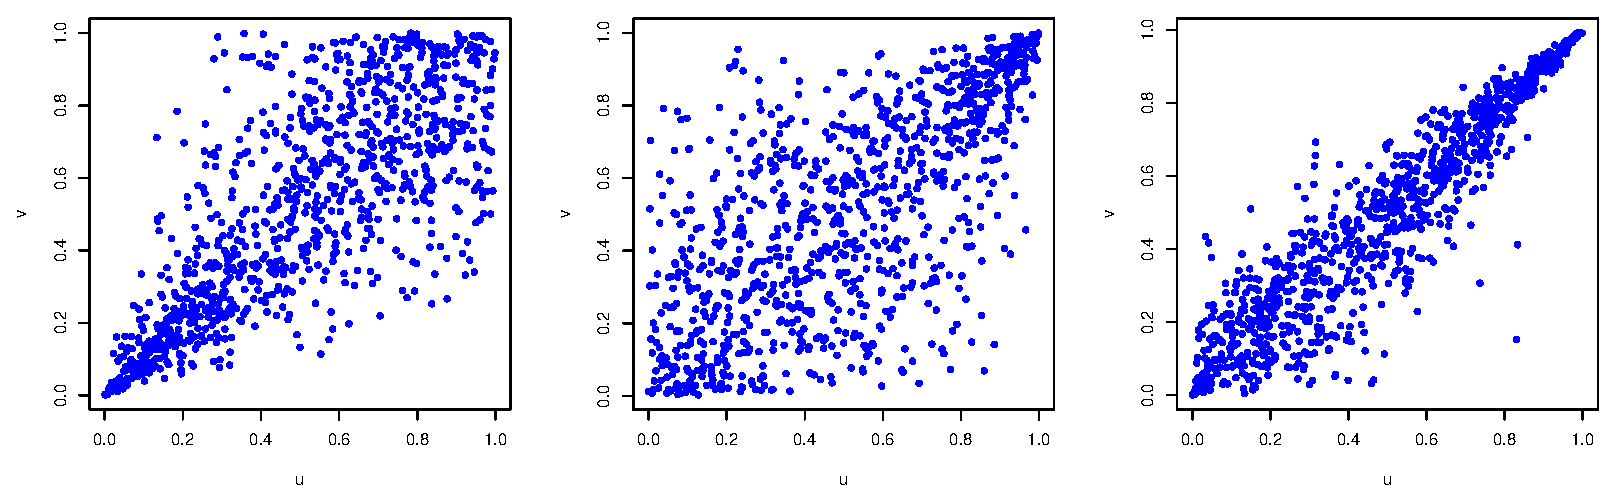
\includegraphics[width=\textwidth]{BB7Scatter.eps}
%   \end{figure}
% \end{frame}

\begin{frame}
  \frametitle{The covariate-contingent copula model}
  %\framesubtitle{The model}
  \begin{itemize}
  \item \textbf{The marginal models}
    \begin{itemize}
    \item In principle, any combination of univariate marginal models can be
      used.
    % \item In the continuous case, we use univariate model that each margin is
    %   from the student \emph{t} distribution.
    \end{itemize}
  \item \textbf{The log likelihood}
    \begin{equation*}
      \begin{split}
        & \log \mathcal{L} (\bm{Y}| \bm{X},\lambda_L, \tau,\bm{\beta}_1,...,\bm{\beta}_M)\\ &=  \sum\nolimits_{i=1}^{n}
        \log c(\bm{u}_1,...,\bm{u}_m, \lambda_L, \tau)\\
& \hspace{1em}  + \sum\nolimits_{m=1}^M \log \mathcal{L}_m(\bm{Y}_m|\bm{X}_m,\bm{\beta}_m)\\
      \end{split}
    \end{equation*}
  \item \textbf{Covariate-dependent structure}

    % where all the parameters are connected with covariates via link function
    % $\varphi(\cdot)$, (identity, log, logit, probit,...)
    \begin{center}
      \begin{tabular}{ll}
        $\bm{\beta}_m = \varphi_{\beta_m}^{-1}(\bm{X}_m\bm{\alpha}_m)$ &$\tau = \varphi_{\tau}^{-1}(X\alpha_{\tau})$ \\
        % $\lambda_L = \varphi_{\lambda}^{-1}((X_u,X_v)\alpha_\lambda)$& $\tau = \varphi_{\tau}^{-1}((X_u,X_v)\alpha_\tau)$ \\
      \end{tabular}
    \end{center}
  \end{itemize}
\end{frame}


\begin{frame}
  \frametitle{The covariate-contingent copula model}
  %\framesubtitle{The priors and posterior}
  \begin{itemize}

  \item The priors

    \begin{itemize}
    \item The priors for the copula functions are easy to specify due to our
      reparameterization.

    \item  The priors for the marginal distributions are specified in their usual
      ways.

    \end{itemize}

  \item The posterior
    \begin{equation*}
      p(\bm{\alpha}|\bm{Y})~ \propto~ \mathcal{L} (\mathbf{Y}| \alpha) \times
      \prod \limits_{i \in \{ {1,..,M,C\}}} p(\alpha_i)
    \end{equation*}

  \item The posterior inference is straightforward although the model is very complicated.

  \end{itemize}
\end{frame}

\begin{frame}
  \frametitle{The covariate-contingent copula model}
  \framesubtitle{Metropolis-Hastings within Gibbs}
  \begin{itemize}
  \item We update all the parameters jointly by using
    Metropolis-Hastings within Gibbs.
  \item The proposal density for each parameter vector $\alpha$ is a multivariate \emph{t}-density with  $df>2$,
    \[
    \bm{\alpha}_{p}|\bm{\alpha}_{c}\sim\bm{MVT}\left[\bm{\hat{\alpha}},~\left.-\left(\frac{\partial^{2}\ln
            p(\bm{\alpha}|\bm{Y})}{\partial\bm{\alpha}\partial\bm{\alpha}^{\prime}}\right)^{-1}\right\vert
      _{\bm{\alpha}=\bm{\hat{\alpha}}},~df\right],
    \]
    where $\bm{\hat{\alpha}}$ is obtained by $R$ steps ($R\leq 3$) Newton's
    iterations during the proposal with analytical gradients.

  \item Variable selections are carried out simultaneously.

  \item \textbf{The key:} The analytical gradients require the derivative for the copula
    density and marginal densities. We implemented it in an efficient way.

  \end{itemize}
\end{frame}

% \section{Example}

% \begin{frame}
%   \frametitle{The covariate-contingent copula model}
%   \framesubtitle{The Joe-Clayton copula}
%   \begin{itemize}
%   \item The Joe-Clayton copula function
%     \[
%     \begin{split}
%       C(u,v,\theta,\delta)=&1-\left[1-\left\{\left(1-\bar u ^{\theta }\right)^{-\delta
%           }+\left(1-\bar v ^{\theta }\right)^{-\delta }-1\right\}^{-1/\delta
%         }\right]^{1/\theta }
%     \end{split}
%     \]
%     where $\theta \geq 1$, $\delta > 0$, $\bar u = 1-u$, $\bar v = 1-v$ .

%   \item Some properties:
%     \begin{itemize}
%     \item One type of Archimedean copula.
%     \item $\lambda_L=2^{-1/\delta}$ does not depend on $\lambda_U=2-2^{-1/\theta}$.
%     \item  $\tau=1- 4\int _0^{\infty} s\times(\varphi'(s))^2ds$ is calculated via Laplace transform.
%     \end{itemize}

%   \item Our interests:
%     \begin{itemize}
%     \item The rank correlation and tail dependence in the model.
%     \item The convenience for interpretation.
%     \end{itemize}

%   \item We use the reparameterized copula    $C(u,v,\lambda_L,
%     \tau)=C(u,v,\theta,\delta)$.
%   \item [*] \textbf{Note!} any other copulas can be equally well used.
%   \end{itemize}

% \end{frame}


% \section{Extensions}
% \begin{frame}
%   \frametitle{Extensions and future work}
%   \begin{itemize}
%   \item More cases (including discrete cases) to be studied in the future.
%   \item It is possible to extend the bivariate copula to multivariate models
%     via various methods, e.g. vine copula, graph model...
%   \item Mixtures of copulas.
%   \end{itemize}
% \end{frame}

\begin{frame}[plain]
  \addtocounter{framenumber}{-1}
  \begin{center}
    {\color{SUblue} \textbf{\Huge Thank you!}}
  \end{center}

    \begin{itemize}

    \item [] For further details, see

      Li, F. (2012), Modeling covariate-contingent correlation and tail-dependence with copulas.
    \end{itemize}

\end{frame}

\end{document}
